\documentclass[12pt]{article}
\usepackage[paperheight=210mm,paperwidth=148mm,top=2cm,bottom=2cm,left=1cm,right=1cm]{geometry}  % A5 paper
\usepackage{background}
\backgroundsetup{
scale=1,
opacity=0.3,
angle=0,
color=black,
contents={%

\includegraphics[width=\paperwidth]{background}
}
}
%%%%%%%%%%%%%%%%%%%%%%%%%%%%%%%%%%%%%%%%
\usepackage[utf8]{inputenc}
\usepackage{titlesec}
%\usepackage[all]{hypcap}
\usepackage{multirow}
%\usepackage{tikz}
\usepackage{ctable}
%%%%%%%%%%%%%%%%%%%%%%%%%%%%%%%%%%%%%%%%
\renewcommand{\familydefault}{\sfdefault}
% \titleformat{\chapter}[display]
% {\bfseries\LARGE\sffamily}{\chaptertitlename}{10pt}{\LARGE}
% \titlespacing*{\chapter}{0pt}{10pt}{10pt}
% \numberwithin{table}{chapter}


\begin{document}
% Cover
\newgeometry{left=0cm, bottom=0cm, top=0cm, right=0cm}
\thispagestyle{empty}
\noindent  % To remove the unwanted white space.
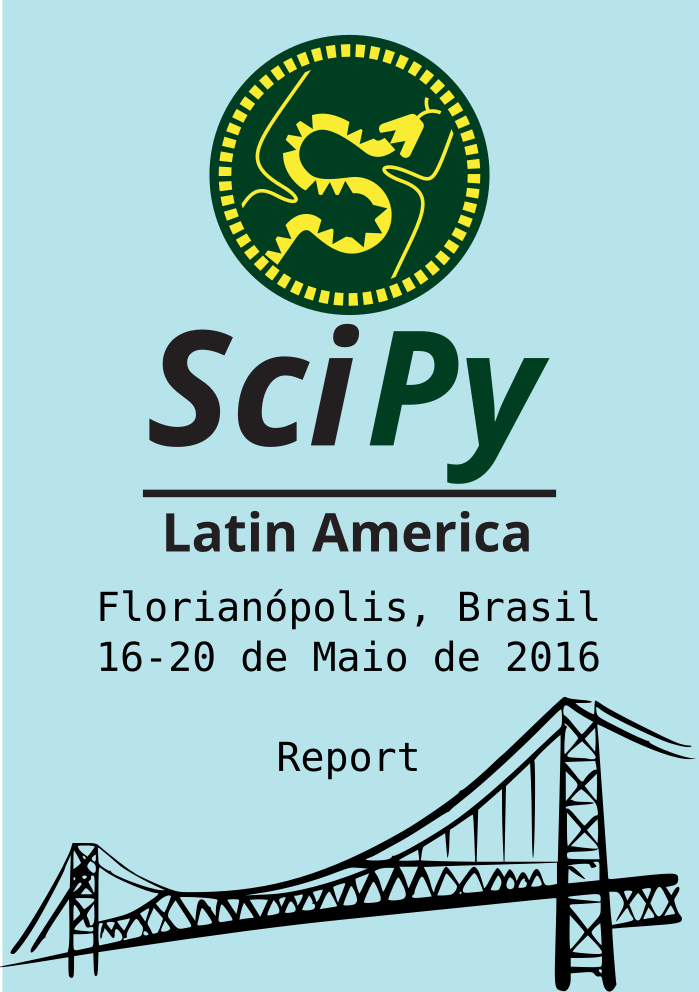
\includegraphics{capa}
\NoBgThispage

\clearpage

\restoregeometry

\newpage

\section*{Map of venue}


\newpage

Hi,

We welcome you to the 4th annual Latin American Conference on Scientific Computing with Python.
This year we will hosting one Software Carpentry workshop for beginners,
12 tutorials, 16 talks, 80 minutes for lightning talks
and some social events that includes an scavenger hunt.

The conference will start with an 40 minutes session for lightning talks
so that attendees could show their pet projects and have three days to talk with
those that will be interested on it.
On the course of the three days you can participate on the scavenger hunt
and try to win it's prize.

We hope that you enjoy your time in Florianópolis.
The Island of Santa Catarina has 42 beaches
and in the case you don't like beaches there is one lagoon.
Try to visit the Public Market
and the Fortress of São José da Ponta Grossa.

\textemdash\ Organizing Committee

\vfill

\hrule

\begin{center}
       \begin{tabular}{p{4cm} p{7cm}}
     Wi-Fi & Website: http://conf.scipyla.org/ \\
     SSID: eduroam & Twitter: http://twitter.com/scipyla/ \\
     Login: scipy & Hashtag: \textbf{\#SciPyLA2016} \\
     Password: SciPyla2016 & \\
   \end{tabular}
\end{center}



\newpage

\section*{Platinum Sponsors}
\begin{minipage}{0.4\textwidth}
COMPANY NAME

FOO

\end{minipage}
\hfill
\begin{minipage}{0.4\textwidth}
COMPANY NAME

FOO

\end{minipage}

\newpage

\section*{Gold Sponsors}
\begin{minipage}{0.4\textwidth}
COMPANY NAME

FOO

\end{minipage}
\hfill
\begin{minipage}{0.4\textwidth}
COMPANY NAME

FOO

\end{minipage}

% Space
\vspace*{1cm}

\begin{minipage}{0.4\textwidth}
COMPANY NAME

FOO

\end{minipage}
\hfill
\begin{minipage}{0.4\textwidth}
COMPANY NAME

FOO

\end{minipage}

\newpage

\section*{Tutorials}

\subsubsection*{16/05/2016}

\begin{center}
   {\footnotesize{%
     \begin{tabular}{@{}l p{5cm} p{5cm}@{}}
     \toprule
      & 9h-12h & 14h-17h\\\midrule
     Room 1 & \textbf{Python for geoscientist} (Filipe Fernandes) & \textbf{Utilización de Vispy para visualización rápida en 3D} (David Ochoa)\\
     Room 2 & \textbf{Introduction to MPI on python using mpi4py} (Jeudy Blanco) & \textbf{Introduction to High-Performance Scientific Computing with PyOpenCL} (Celia Cintas)\\
     Auditorium & \textbf{I see 42 everywhere} (Fernando Masanori) & \textbf{The stupid content tracker} (Tomas Aliaga)\\\bottomrule
   \end{tabular}
 }}
\end{center}

\subsubsection*{17/05/2016}

\begin{center}
   {\footnotesize{%
     \begin{tabular}{@{}l p{5cm} p{5cm}@{}}
     \toprule
      & 9h-12h & 14h-17h\\\midrule
     Room 1 & \textbf{Fit and predict your data: Introduction to Scikit-learn} (Celia Cintas) & \textbf{scikit-image: Realce e Detecção de bordas$^\star$} (Darleison Rodrigues)\\
     Room 2 & \textbf{Scientific Python applied to Petroleum Engineering - an Introduction$^\star$} (Igor T. Ghisi) & \textbf{Time Series Analysis Using Python$^\star$} (Bargava Subramanian)\\
     Auditorium & \textbf{Introduction to Data Analysis using Python Data Stack$^\star$} (Bargava Subramanian) & \textbf{Usando R com o Python - rpy2$^\star$} (Arnaldo Russo)\\\bottomrule
   \end{tabular}
 }}
\end{center}
{\footnotesize{$^\star$ Waiting for confirmation.}}

\subsubsection*{Locations}
{\footnotesize{%
\begin{description}
   \item[Room 1] Sala de Projeção Harry Laus (40)
   \item[Room 2] Sala de Projeção Henrique da Silva Fontes (24)
   \item[Auditorium] Auditório Elke Hering (80)
\end{description}
}}


\subsection*{List of tutorials}
\begin{description}
   \item[16/05/2016] \ 
   \begin{itemize}
      \item \textbf{Python for geoscientist}, \emph{Filipe Fernandes (ocefpaf@gmail.com)}. Intermediate. Sala de projeção Harry Laus, 9h-12h.
      \item \textbf{Utilización de Vispy para visualización rápida en 3D}, \emph{David Ochoa (ochoadavid@gmail.com)}. Intermediate. Sala de Projeção Harry Laus, 14h-17h.
      \item \textbf{Introduction to MPI on python using mpi4py}, \emph{Jeudy Blanco (jeudyx@gmail.com)}. Introductory. Sala de Projeção Henrique da Silva Fontes, 9h-12h.
      \item \textbf{Introduction to High-Performance Scientific Computing with PyOpenCL}, \emph{Celia Cintas (cintas.celia@gmail.com)}. Introductory. Sala de Projeção Henrique da Silva Fontes, 14h-17h.
      \item \textbf{I see 42 everywhere}, \emph{Fernando Masanori (fmasanori@gmail.com)}. Introductory. Auditório Elke Hering, 9h-12h.
      \item \textbf{The stupid content tracker}, \emph{Tomas Aliaga (tomas.aliaga@gmail.com)}. Introductory. Auditório Elke Hering, 14h-17h.
   \end{itemize}
   \item[17/05/2016] \ 
   \begin{itemize}
      \item \textbf{Fit and predict your data: Introduction to Scikit-learn}, \emph{Celia Cintas (cintas.celia@gmail.com)}. Introductory. Sala de Projeção Harry Laus, 9h-12h.
      \item \textbf{scikit-image: Realce e Detecção de bordas}, \emph{Darleison Rodrigues (darleison.f@gmail.com)}. Intermediate. Sala de Projeção Harry Laus, 14h-17h. \underline{(Waiting for confirmation)}
      \item \textbf{Scientific Python applied to Petroleum Engineering - an Introduction}, \emph{Igor T. Ghisi (igortg.subs@gmail.com)}. Introductory. Sala de Projeção Henrique da Silva Fontes, 9h-12h. \underline{(Waiting for confirmation)} 
      \item \textbf{Time Series Analysis Using Python}, \emph{Bargava Subramanian (bargava@gmail.com)}. Introductory. Sala de Projeção Henrique da Silva Fontes, 14h-17h. \underline{(Waiting for confirmation)}
      \item \textbf{Introduction to Data Analysis using Python Data Stack}, \emph{Bargava Subramanian (bargava@gmail.com)}. Introductory. Auditório Elke Hering, 9h-12h. \underline{(Waiting for confirmation)}
    \item \textbf{Usando R com o Python - rpy2}, \emph{Arnaldo Russo (arnaldorusso@gmail.com)}. Intermediate. Auditório Elke Hering, 14h-17h. \underline{(Waiting for confirmation)}
   \end{itemize}
\end{description}

\newpage

% Last Page
\vspace*{1cm}

\end{document}
